% 1
\subsection{Parks}

\subsubsection{IOI\,2021 D1T3 (loj\,3525)}

\frame {\vspace{20pt}
	给定平面上 $n$ 个互不相同且坐标形如 $(2 x_i, 2 y_i)$ ($x_i, y_i \in \f Z$) 的点,\!每对距离为 $2$ 的点之间连有一条边,\!保证所得的图 $G$ 连通。

	你需要构造 $G$ 的一棵生成树 $T = (V, E)$,同时构造 $n - 1$ 个不同的形如 $(2 x_i \!+\! 1, 2 y_i \!+\! 1)$ ($x_i, y_i \!\in\! \f Z$) 的点,使得存在这些点到 $E$ 的一一映射 $\varphi$ 使得 $p$ 和 $\varphi(p)$ 的两端点构成等腰直角三角形。

	{\color{fuchsia}$1 \leq n \leq 2 \times 10^5$。}

	\begin{figure}[htb]
		\centering
		\begin{tikzpicture}[x=.33cm, y=.33cm]
			\useasboundingbox (0, -0.4) rectangle (8, 7.6);
			\onlyx<2>{
				\fill[nearly opaque, white] (-1.25, -1) rectangle (9, 9.25);
				\draw[help lines, step=2] (0, 0) grid (8, 8);
				\draw[->] (-0.5, 0) -- (8, 0) node[right, inner sep=3pt] {\footnotesize $x$};
				\draw[->] (0, -0.5) -- (0, 8) node[above, inner sep=3pt] {\footnotesize $y$};
				\begin{scope}[blue, circle, minimum size=2.5pt, every node/.style=fill]
					\node (W) at (2, 4) {};
					\node (E) at (6, 4) {};
					\node (N) at (4, 6) {};
					\node (S) at (4, 2) {};
					\node (C) at (4, 4) {};
				\end{scope}
				\begin{scope}[red, minimum size=2.5pt, every node/.style=draw]
					\node (NW) at (3, 5) {};
					\node (NE) at (5, 5) {};
					\node (SW) at (3, 3) {};
					\node (SE) at (5, 3) {};
				\end{scope}
				\draw[blue] (W) -- (E) (N) -- (S);
				\draw[densely dotted] (NW) -- (NW -| N) (NE) -- (NE |- E) (SE) -- (SE -| S) (SW) -- (SW |- W);
				\node foreach \x in {2, 4, 6} [below, inner sep=3pt] at (\x, 0) {\footnotesize $\x$};
				\node foreach \y in {2, 4, 6} [left, inner sep=3pt] at (0, \y) {\footnotesize $\y$};
			}
			\draw[->, fuchsia, rounded corners=.25cm] (-2, 19.75) -- (-2, 21.35) -- (-12.5, 21.35);
			\node at (-2, 19.25) {\tiny\color{fuchsia}题目名称};
			\draw[->, fuchsia, rounded corners=.25cm] (14.25, 19.25) -- (15.75, 19.25) -- (15.75, 20.75);
			\node at (12.75, 19.25) {\tiny\color{fuchsia}题目来源};
		\end{tikzpicture}
		\onslidex<2>{\caption{}}
	\end{figure}
}

\sol {\vspace{12pt}
	\compress{-4pt}{考虑将坐标系旋转 $45^\circ$,\!所有点可以根据新的 $y$ 坐标两两配对。}

	\onslide<2->{\compress{-4pt}{对于同一层的点,\!可以将其连接并选择其右侧的点与之对应。}}

	\onslide<3->{对于不同层的点,考虑连通其的边,对于固定的两个连通块,我们考虑连接其的边中\textsl{最靠左}的那条,并选择其左侧的点与之对应。}

	\begin{figure}[htb]
		\centering
		\begin{tikzpicture}[x=.4cm, y=.4cm]
			\useasboundingbox (-4.6, -3.5) rectangle (7.4, 4);
			\clip (-4.6, -3.5) rectangle (7.4, 5);
			\fill[nearly opaque, white] (-5, -4) rectangle (8, 6);
			\fill[nearly transparent, blue] (-5, 2.357) rectangle (8, 4.714);
			\fill[nearly transparent, fuchsia] (-5, -0.4714) rectangle (8, 1.886);
			\fill[nearly transparent, blue] (-5, -3.3) rectangle (8, -0.9428);
			\begin{scope}[rotate=45]
				\draw[help lines, step=2] (-8, -8) grid (10, 8);
				\begin{scope}[circle, minimum size=2.5pt, every node/.style=fill]
					\begin{scope}[blue]
						\node (A) at (0, 4) {};
						\node (B) at (2, 4) {};
						\node (C) at (2, 2) {};
						\node (D) at (4, 2) {};
						\node (E) at (6, 0) {};
						\node (F) at (6, -2) {};
					\end{scope}
					\begin{scope}[fuchsia]
						\node (G) at (0, 2) {};
						\node (H) at (0, 0) {};
						\node (I) at (2, 0) {};
						\node (J) at (4, -2) {};
						\node (K) at (4, -4) {};
					\end{scope}
					\begin{scope}[blue]
						\node (L) at (-2, 0) {};
						\node (M) at (0, -2) {};
						\node (N) at (0, -4) {};
						\node (O) at (2, -4) {};
					\end{scope}
				\end{scope}
				\only<2->{
					\draw[blue] (A) -- (B) -- (C) -- (D) (E) -- (F) (M) -- (N) -- (O);
					\draw[fuchsia] (G) -- (H) -- (I) (J) -- (K);
					\begin{scope}[red, minimum size=2.5pt, every node/.style=draw]
						\node (a) at (1, 3) {};
						\node (b) at (3, 3) {};
						\node (c) at (3, 1) {};
						\node (d) at (7, -1) {};
						\node (e) at (1, 1) {};
						\node (f) at (1, -1) {};
						\node (g) at (5, -3) {};
						\node (h) at (1, -3) {};
						\node (i) at (1, -5) {};
					\end{scope}
					\begin{scope}[->]
						\draw (a) -- (a |- A);
						\draw (b) -- (b -| B);
						\draw (c) -- (c |- C);
						\draw (d) -- (d -| E);
						\draw (e) -- (e -| G);
						\draw (f) -- (f |- H);
						\draw (g) -- (g -| J);
						\draw (h) -- (h -| M);
						\draw (i) -- (i |- N);
					\end{scope}
				}
				\only<3->{
					\draw[semithick, properpurple] (A) -- (G) (F) -- (J) (H) -- (L) (H) -- (M) (K) -- (O);
					\begin{scope}[orange, minimum size=2.5pt, every node/.style=draw]
						\node (ag) at (-1, 3) {};
						\node (fj) at (5, -1) {};
						\node (hl) at (-1, 1) {};
						\node (hm) at (-1, -1) {};
						\node (ko) at (3, -3) {};
					\end{scope}
					\begin{scope}[->]
						\draw (ag) -- (ag -| A);
						\draw (fj) -- (fj |- F);
						\draw (hl) -- (hl |- H);
						\draw (hm) -- (hm -| H);
						\draw (ko) -- (ko |- K);
					\end{scope}
				}
			\end{scope}
		\end{tikzpicture}
	\end{figure}
}

% 2
\subsection{挑战哈密顿 2}

\subsubsection{原创题}

\frame {\vspace{20pt}
	给定无向简单图 $G \mathbin= (V, E)$,其中 $V \mathbin= \bigl\{ (i, j) \bigm| 0 \mathbin\leq i \mathbin\leq C - 1, \break \text{$0 \leq j \leq R - 1$ 且 $i, j$ 为整数} \bigr\}$,$E$ 为所有距离为 $1$ 或 $\sqrt 2$ 的点对构成的二元组。你需要找到 $G$ 的一个 Hamilton 圈,满足:
	\begin{itemize}
		\item \compress{-24pt}{该圈的任意\textsl{连续}两条边不平行 (等价地,任意连续三点不共线);}
		\item (\textsl{视每条边为直线段}) 任意两条边不在非顶点处相交。
	\end{itemize}
	或说明其不存在。{\color{fuchsia}$R \times C \leq 10^6$。}\pausex

	\begin{figure}
		\centering
		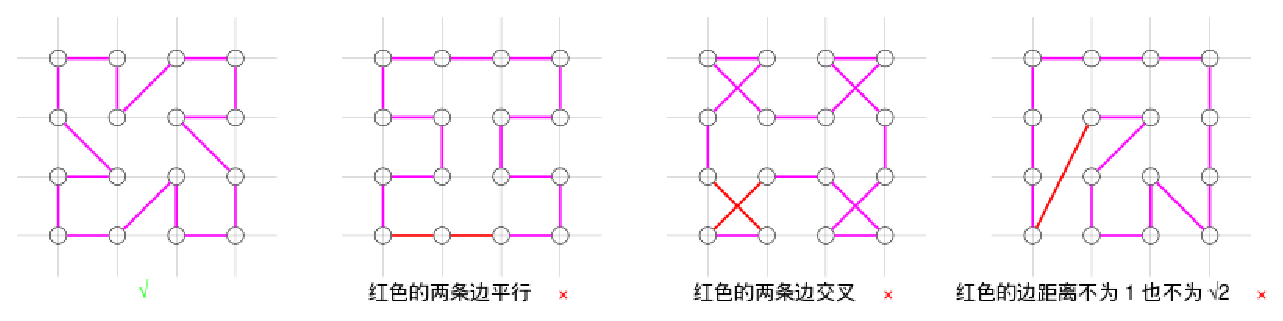
\includegraphics[scale=.4]{assets/hamilton}
		\caption{}
	\end{figure}
}

\sol {\vspace{20pt}
	不妨设 $R \leq C$。容易证明当 $R \leq 3$ 时除 $(R, C) = (2, 2)$ 有平凡解外其余情况都无解,暴搜知 $(R, C) = (5, 5)$ 时无解。\pause

	其余情况均可构造解。我们增强条件,希望从 $(0, 0)$ 开始的前两步分别是右、上。根据下图可知我们可以从 $(R, C)$ 的答案归纳得到 $(R + 4, C + 4)$ 的答案。\pause

	\begin{figure}
		\centering
		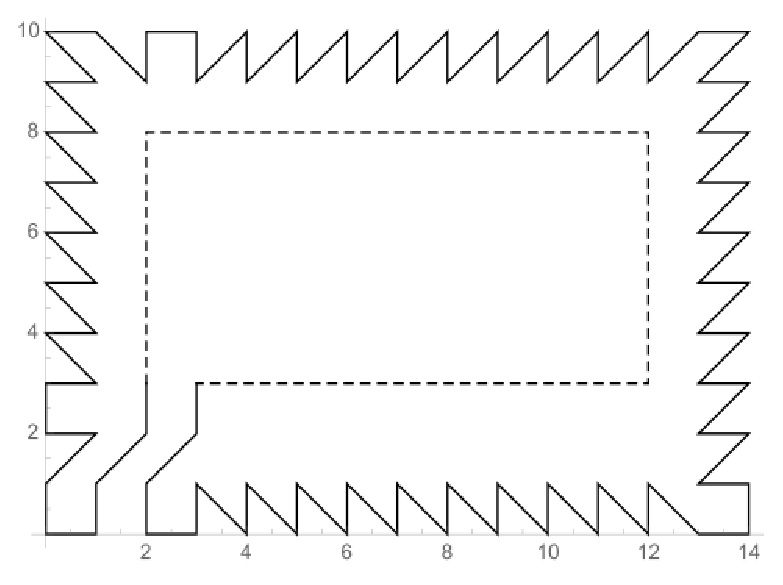
\includegraphics[scale=.35]{assets/enlarge4}
		\caption{}
	\end{figure}
}

\sol {
	于是只需考虑 $4 \leq R \leq 7$ 的情形以及 $(R, C) = (9, 9)$。这些情况可以通过手玩、搜索等方法来完成。
}

% 3
\subsection{Pattern Lock (改编版)}

\subsubsection{JSCPC\,2021\,D (Codeforces\,Gym 103495\,D)}

\frame {\vspace{20pt}
	给定\textsl{完全图} $G = (V, E)$,其中 $V = \bigl\{ (i, j) \bigm| 0 \leq i \leq C - 1, \break \text{$0 \leq j \leq R - 1$ 且 $i, j$ 为整数} \bigr\}$。你需要找到 $G$ 的一个 Hamilton 圈,满足\textsl{视每条边为直线段}后:
	\begin{itemize}
		\item 对任意点 $v \in V$,它关联的两条边构成一个锐角。
		\item 每一条边不能经过除端点外的其它顶点。
	\end{itemize}
	或说明其不存在。{\color{fuchsia}$R \times C \leq 10^6$。}\pausex

	\begin{figure}[htb]
		\centering
		\begin{tikzpicture}
			\fill[nearly opaque, white] (-0.35, -0.35) rectangle (1.35, 1.35);
			\draw[help lines, step=1] (-0.35, -0.35) grid (1.35, 1.35);
			\begin{scope}[circle, minimum size=6pt, every node/.style=draw]
				\node (A) at (0, 0) {};
				\node (B) at (1, 0) {};
				\node (C) at (0, 1) {};
				\node (D) at (1, 1) {};
			\end{scope}
			\draw[semithick, fuchsia] (A) -- (B) -- (C) -- (D) -- (A);
		\end{tikzpicture}
		\caption{}
	\end{figure}
}

\sol {\vspace{12pt}
	\compress{-4pt}{故技重施。\!仍然考虑通过 $(R, C)$ 的解得到 $(R + 4, C + 4)$ 的解。}\pause

	\begin{figure}[htb]
		\centering
		\begin{tikzpicture}[x=.6cm, y=.6cm]
			\fill[nearly opaque, white] (-0.5, -0.5) rectangle (12.5, 8.5);
			\draw[help lines, step=1] (-0.5, -0.5) grid (12.5, 8.5);
			\begin{scope}[circle, minimum size=3pt]
				\node foreach \x in {0,...,12} foreach \y in {0,...,8} [draw] (\x v\y) at (\x, \y) {};
			\end{scope}
			\draw[fuchsia]
					(4v8) -- (4v7) -- (5v8) -- (5v7) -- (6v8) -- (6v7) -- (7v8) -- (7v7)
				 -- (8v8) -- (8v7) -- (9v8) -- (9v7) -- (10v8) -- (10v7) -- (12v8) -- (11v8)
				 -- (12v7) -- (11v7) -- (12v6) -- (11v6) -- (12v5) -- (11v5) -- (12v4) -- (11v4)
				 -- (12v3) -- (11v3) -- (12v2) -- (11v2) -- (12v0) -- (12v1) -- (11v0) -- (11v1)
				 -- (10v0) -- (10v1) -- (9v0) -- (9v1) -- (8v0) -- (8v1) -- (7v0) -- (7v1)
				 -- (6v0) -- (6v1) -- (5v0) -- (5v1) -- (4v0) -- (4v1) -- (3v0) -- (3v1)
				 -- (2v0) -- (2v1) -- (0v0) -- (1v0) -- (0v1) -- (1v1) -- (0v2) -- (1v2)
				 -- (0v3) -- (1v3) -- (0v4) -- (1v4) -- (0v5) -- (1v5) -- (0v6) -- (1v6)
				 -- (0v8) -- (0v7);
			\only<2-3>{
				\draw[fuchsia] (0v7) -- (1v8) -- (1v7) -- (2v8) -- (2v7) -- (3v8) -- (3v7) -- (4v8);
			}
			\only<3>{
				\draw[red] (2v2) -- (3v2);
			}
			\only<3->{
				\draw[red, dash pattern=on 1.5pt off 1.5pt] (2v2) -- (2.666667, 3.666667) (3v2) -- (2.333333, 3.666667);
			}
			\only<4->{
				\draw[semithick, blue] (2v2) -- (3v8);
				\draw[semithick, blue] (3v2) -- (4v8);
				\draw[fuchsia] (1v8) -- (1v7) -- (2v8) (2v7) -- (3v8);
				\draw[semithick, orange] (0v7) -- (2v8) (1v8) -- (3v7) -- (2v7);
			}
		\end{tikzpicture}
	\end{figure}
}
